\documentclass{standalone}
\usepackage{tikz}
\usetikzlibrary{patterns, positioning}


\begin{document}
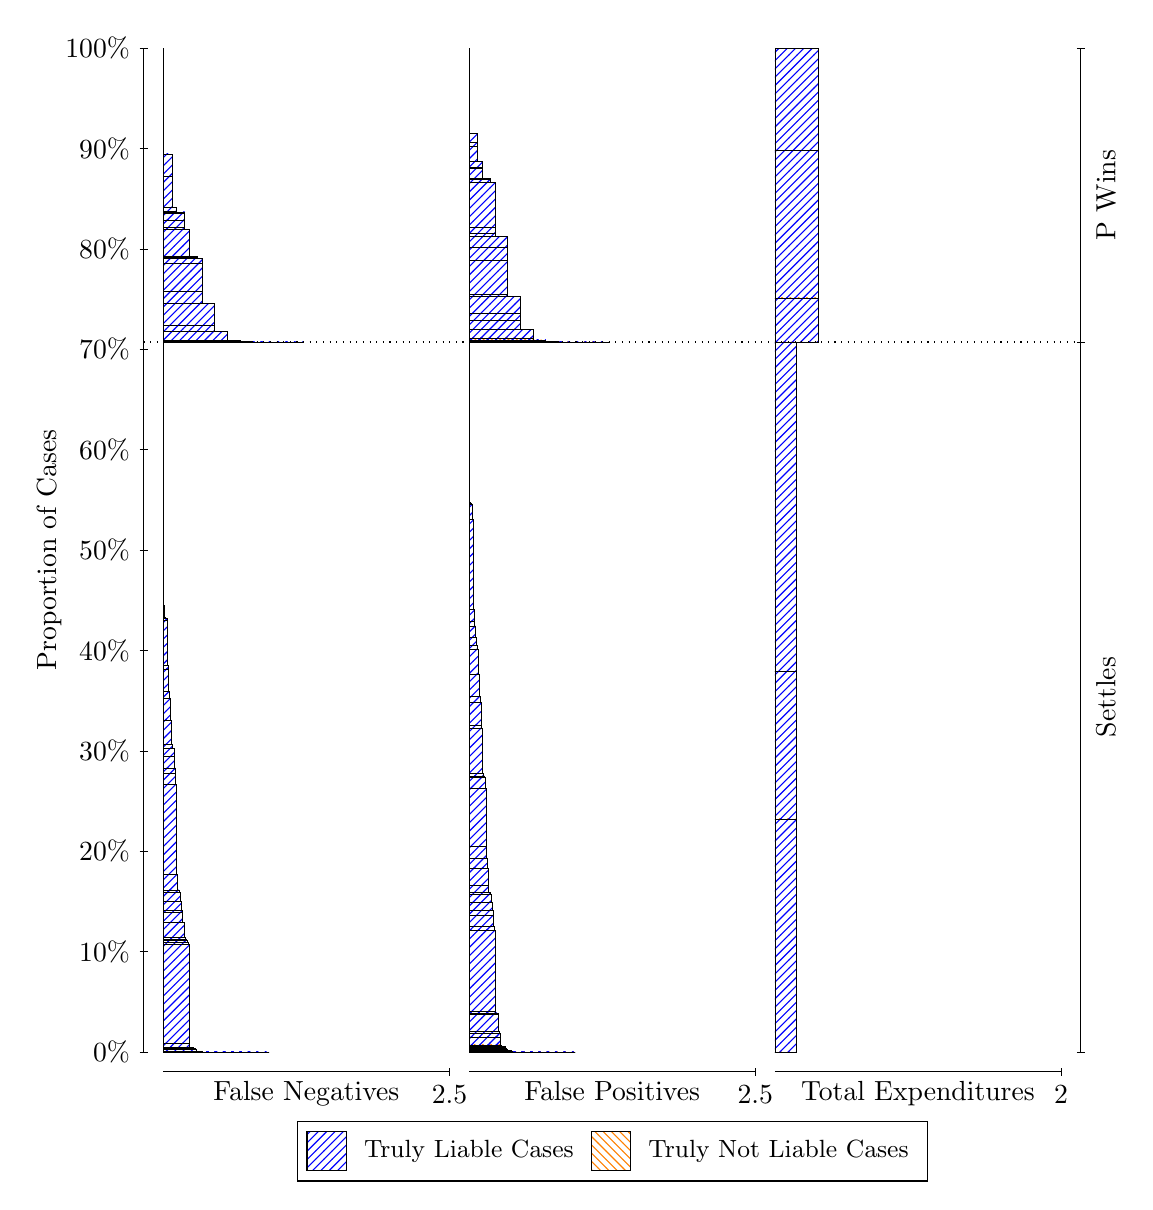
\begin{tikzpicture}
\draw[black, very thin] (1.5,1.75) -- (1.5,14.5);
\node[rotate=90, text=black, anchor=center] at (0.3, 8.125) {Proportion of Cases};
\draw[black, very thin] (1.45,1.75) -- (1.55,1.75);
\node[text=black, anchor=east] at (1.45, 1.75) {0\%};
\draw[black, very thin] (1.45,3.025) -- (1.55,3.025);
\node[text=black, anchor=east] at (1.45, 3.025) {10\%};
\draw[black, very thin] (1.45,4.3) -- (1.55,4.3);
\node[text=black, anchor=east] at (1.45, 4.3) {20\%};
\draw[black, very thin] (1.45,5.575) -- (1.55,5.575);
\node[text=black, anchor=east] at (1.45, 5.575) {30\%};
\draw[black, very thin] (1.45,6.85) -- (1.55,6.85);
\node[text=black, anchor=east] at (1.45, 6.85) {40\%};
\draw[black, very thin] (1.45,8.125) -- (1.55,8.125);
\node[text=black, anchor=east] at (1.45, 8.125) {50\%};
\draw[black, very thin] (1.45,9.4) -- (1.55,9.4);
\node[text=black, anchor=east] at (1.45, 9.4) {60\%};
\draw[black, very thin] (1.45,10.675) -- (1.55,10.675);
\node[text=black, anchor=east] at (1.45, 10.675) {70\%};
\draw[black, very thin] (1.45,11.95) -- (1.55,11.95);
\node[text=black, anchor=east] at (1.45, 11.95) {80\%};
\draw[black, very thin] (1.45,13.225) -- (1.55,13.225);
\node[text=black, anchor=east] at (1.45, 13.225) {90\%};
\draw[black, very thin] (1.45,14.5) -- (1.55,14.5);
\node[text=black, anchor=east] at (1.45, 14.5) {100\%};

\draw[black, very thin] (13.4,1.75) -- (13.4,14.5);
\draw[black, very thin] (13.35,1.75) -- (13.45,1.75);
\node[anchor=west] at (13.35, 1.75) {};
\draw[black, very thin] (13.35,10.767) -- (13.45,10.767);
\node[anchor=west] at (13.35, 10.767) {};
\draw[black, very thin] (13.35,14.5) -- (13.45,14.5);
\node[anchor=west] at (13.35, 14.5) {};

\draw[black, very thin, pattern color=blue, pattern=north east lines] (1.75,1.75) rectangle (3.0943,1.75);
\draw[black, very thin, pattern color=blue, pattern=north east lines] (1.75,1.75) rectangle (3.0217,1.75);
\draw[black, very thin, pattern color=blue, pattern=north east lines] (1.75,1.75) rectangle (2.949,1.75);
\draw[black, very thin, pattern color=blue, pattern=north east lines] (1.75,1.75) rectangle (2.9329,1.75);
\draw[black, very thin, pattern color=blue, pattern=north east lines] (1.75,1.75) rectangle (2.8763,1.75);
\draw[black, very thin, pattern color=blue, pattern=north east lines] (1.75,1.75) rectangle (2.8602,1.75);
\draw[black, very thin, pattern color=blue, pattern=north east lines] (1.75,1.75) rectangle (2.8037,1.75);
\draw[black, very thin, pattern color=blue, pattern=north east lines] (1.75,1.75) rectangle (2.7875,1.75);
\draw[black, very thin, pattern color=blue, pattern=north east lines] (1.75,1.75) rectangle (2.7714,1.75);
\draw[black, very thin, pattern color=blue, pattern=north east lines] (1.75,1.75) rectangle (2.731,1.75);
\draw[black, very thin, pattern color=blue, pattern=north east lines] (1.75,1.75) rectangle (2.7149,1.75);
\draw[black, very thin, pattern color=blue, pattern=north east lines] (1.75,1.75) rectangle (2.6987,1.75);
\draw[black, very thin, pattern color=blue, pattern=north east lines] (1.75,1.75) rectangle (2.6583,1.75);
\draw[black, very thin, pattern color=blue, pattern=north east lines] (1.75,1.75) rectangle (2.6422,1.75);
\draw[black, very thin, pattern color=blue, pattern=north east lines] (1.75,1.75) rectangle (2.626,1.75);
\draw[black, very thin, pattern color=blue, pattern=north east lines] (1.75,1.75) rectangle (2.6099,1.75);
\draw[black, very thin, pattern color=blue, pattern=north east lines] (1.75,1.75) rectangle (2.5857,1.75);
\draw[black, very thin, pattern color=blue, pattern=north east lines] (1.75,1.75) rectangle (2.5695,1.75);
\draw[black, very thin, pattern color=blue, pattern=north east lines] (1.75,1.75) rectangle (2.5534,1.75);
\draw[black, very thin, pattern color=blue, pattern=north east lines] (1.75,1.75) rectangle (2.5372,1.75);
\draw[black, very thin, pattern color=blue, pattern=north east lines] (1.75,1.75) rectangle (2.513,1.75);
\draw[black, very thin, pattern color=blue, pattern=north east lines] (1.75,1.75) rectangle (2.4969,1.75);
\draw[black, very thin, pattern color=blue, pattern=north east lines] (1.75,1.75) rectangle (2.4807,1.75);
\draw[black, very thin, pattern color=blue, pattern=north east lines] (1.75,1.75) rectangle (2.4646,1.75);
\draw[black, very thin, pattern color=blue, pattern=north east lines] (1.75,1.75) rectangle (2.4484,1.75);
\draw[black, very thin, pattern color=blue, pattern=north east lines] (1.75,1.75) rectangle (2.4403,1.75);
\draw[black, very thin, pattern color=blue, pattern=north east lines] (1.75,1.75) rectangle (2.4242,1.75);
\draw[black, very thin, pattern color=blue, pattern=north east lines] (1.75,1.75) rectangle (2.408,1.75);
\draw[black, very thin, pattern color=blue, pattern=north east lines] (1.75,1.75) rectangle (2.3919,1.75);
\draw[black, very thin, pattern color=blue, pattern=north east lines] (1.75,1.75) rectangle (2.3757,1.75);
\draw[black, very thin, pattern color=blue, pattern=north east lines] (1.75,1.75) rectangle (2.3677,1.75);
\draw[black, very thin, pattern color=blue, pattern=north east lines] (1.75,1.75) rectangle (2.3515,1.75);
\draw[black, very thin, pattern color=blue, pattern=north east lines] (1.75,1.75) rectangle (2.3354,1.7506);
\draw[black, very thin, pattern color=blue, pattern=north east lines] (1.75,1.7506) rectangle (2.3192,1.7507);
\draw[black, very thin, pattern color=blue, pattern=north east lines] (1.75,1.7507) rectangle (2.3031,1.7508);
\draw[black, very thin, pattern color=blue, pattern=north east lines] (1.75,1.7508) rectangle (2.295,1.7508);
\draw[black, very thin, pattern color=blue, pattern=north east lines] (1.75,1.7508) rectangle (2.2869,1.7508);
\draw[black, very thin, pattern color=blue, pattern=north east lines] (1.75,1.7508) rectangle (2.2789,1.7508);
\draw[black, very thin, pattern color=blue, pattern=north east lines] (1.75,1.7508) rectangle (2.2627,1.7509);
\draw[black, very thin, pattern color=blue, pattern=north east lines] (1.75,1.7509) rectangle (2.2466,1.7532);
\draw[black, very thin, pattern color=blue, pattern=north east lines] (1.75,1.7532) rectangle (2.2304,1.7538);
\draw[black, very thin, pattern color=blue, pattern=north east lines] (1.75,1.7538) rectangle (2.2223,1.7543);
\draw[black, very thin, pattern color=blue, pattern=north east lines] (1.75,1.7543) rectangle (2.2143,1.7547);
\draw[black, very thin, pattern color=blue, pattern=north east lines] (1.75,1.7547) rectangle (2.2062,1.7554);
\draw[black, very thin, pattern color=blue, pattern=north east lines] (1.75,1.7554) rectangle (2.19,1.7566);
\draw[black, very thin, pattern color=blue, pattern=north east lines] (1.75,1.7566) rectangle (2.1739,1.78);
\draw[black, very thin, pattern color=blue, pattern=north east lines] (1.75,1.78) rectangle (2.1577,1.7894);
\draw[black, very thin, pattern color=blue, pattern=north east lines] (1.75,1.7894) rectangle (2.1497,1.7937);
\draw[black, very thin, pattern color=blue, pattern=north east lines] (1.75,1.7937) rectangle (2.1416,1.8003);
\draw[black, very thin, pattern color=blue, pattern=north east lines] (1.75,1.8003) rectangle (2.1335,1.8005);
\draw[black, very thin, pattern color=blue, pattern=north east lines] (1.75,1.8005) rectangle (2.1254,1.8061);
\draw[black, very thin, pattern color=blue, pattern=north east lines] (1.75,1.8061) rectangle (2.1174,1.807);
\draw[black, very thin, pattern color=blue, pattern=north east lines] (1.75,1.807) rectangle (2.1012,1.8089);
\draw[black, very thin, pattern color=blue, pattern=north east lines] (1.75,1.8089) rectangle (2.0851,1.8572);
\draw[black, very thin, pattern color=blue, pattern=north east lines] (1.75,1.8572) rectangle (2.077,3.1161);
\draw[black, very thin, pattern color=blue, pattern=north east lines] (1.75,3.1161) rectangle (2.0689,3.1397);
\draw[black, very thin, pattern color=blue, pattern=north east lines] (1.75,3.1397) rectangle (2.0609,3.1481);
\draw[black, very thin, pattern color=blue, pattern=north east lines] (1.75,3.1481) rectangle (2.0528,3.1686);
\draw[black, very thin, pattern color=blue, pattern=north east lines] (1.75,3.1686) rectangle (2.0447,3.1858);
\draw[black, very thin, pattern color=blue, pattern=north east lines] (1.75,3.1858) rectangle (2.0286,3.2056);
\draw[black, very thin, pattern color=blue, pattern=north east lines] (1.75,3.2056) rectangle (2.0124,3.3993);
\draw[black, very thin, pattern color=blue, pattern=north east lines] (1.75,3.3993) rectangle (1.9963,3.522);
\draw[black, very thin, pattern color=blue, pattern=north east lines] (1.75,3.522) rectangle (1.9882,3.552);
\draw[black, very thin, pattern color=blue, pattern=north east lines] (1.75,3.552) rectangle (1.9801,3.659);
\draw[black, very thin, pattern color=blue, pattern=north east lines] (1.75,3.659) rectangle (1.972,3.666);
\draw[black, very thin, pattern color=blue, pattern=north east lines] (1.75,3.666) rectangle (1.964,3.784);
\draw[black, very thin, pattern color=blue, pattern=north east lines] (1.75,3.784) rectangle (1.9559,3.7974);
\draw[black, very thin, pattern color=blue, pattern=north east lines] (1.75,3.7974) rectangle (1.9397,3.8098);
\draw[black, very thin, pattern color=blue, pattern=north east lines] (1.75,3.8098) rectangle (1.9236,4.0027);
\draw[black, very thin, pattern color=blue, pattern=north east lines] (1.75,4.0027) rectangle (1.9155,5.1486);
\draw[black, very thin, pattern color=blue, pattern=north east lines] (1.75,5.1486) rectangle (1.9074,5.2924);
\draw[black, very thin, pattern color=blue, pattern=north east lines] (1.75,5.2924) rectangle (1.8994,5.3569);
\draw[black, very thin, pattern color=blue, pattern=north east lines] (1.75,5.3569) rectangle (1.8913,5.5063);
\draw[black, very thin, pattern color=blue, pattern=north east lines] (1.75,5.5063) rectangle (1.8832,5.6044);
\draw[black, very thin, pattern color=blue, pattern=north east lines] (1.75,5.6044) rectangle (1.8671,5.6586);
\draw[black, very thin, pattern color=blue, pattern=north east lines] (1.75,5.6586) rectangle (1.8509,5.9667);
\draw[black, very thin, pattern color=blue, pattern=north east lines] (1.75,5.9667) rectangle (1.8348,6.247);
\draw[black, very thin, pattern color=blue, pattern=north east lines] (1.75,6.247) rectangle (1.8267,6.3303);
\draw[black, very thin, pattern color=blue, pattern=north east lines] (1.75,6.3303) rectangle (1.8186,6.6139);
\draw[black, very thin, pattern color=blue, pattern=north east lines] (1.75,6.6139) rectangle (1.8106,6.6578);
\draw[black, very thin, pattern color=blue, pattern=north east lines] (1.75,6.6578) rectangle (1.8025,7.229);
\draw[black, very thin, pattern color=blue, pattern=north east lines] (1.75,7.229) rectangle (1.7944,7.2619);
\draw[black, very thin, pattern color=blue, pattern=north east lines] (1.75,7.2619) rectangle (1.7783,7.2754);
\draw[black, very thin, pattern color=blue, pattern=north east lines] (1.75,7.2754) rectangle (1.7621,7.4234);
\draw[black, very thin, pattern color=blue, pattern=north east lines] (1.75,7.4234) rectangle (1.754,8.1602);
\draw[black, very thin, pattern color=orange, pattern=north west lines] (1.75,8.1602) rectangle (1.75,8.1602);
\draw[black, very thin, pattern color=blue, pattern=north east lines] (1.75,8.1602) rectangle (1.75,10.767);
\draw[black, very thin, pattern color=blue, pattern=north east lines] (1.75,10.767) rectangle (3.5303,10.767);
\draw[black, very thin, pattern color=blue, pattern=north east lines] (1.75,10.767) rectangle (3.3689,10.767);
\draw[black, very thin, pattern color=blue, pattern=north east lines] (1.75,10.767) rectangle (3.2074,10.767);
\draw[black, very thin, pattern color=blue, pattern=north east lines] (1.75,10.767) rectangle (3.0459,10.767);
\draw[black, very thin, pattern color=blue, pattern=north east lines] (1.75,10.767) rectangle (2.9894,10.767);
\draw[black, very thin, pattern color=blue, pattern=north east lines] (1.75,10.767) rectangle (2.8844,10.769);
\draw[black, very thin, pattern color=blue, pattern=north east lines] (1.75,10.769) rectangle (2.8844,10.77);
\draw[black, very thin, pattern color=blue, pattern=north east lines] (1.75,10.77) rectangle (2.8279,10.77);
\draw[black, very thin, pattern color=blue, pattern=north east lines] (1.75,10.77) rectangle (2.7229,10.779);
\draw[black, very thin, pattern color=blue, pattern=north east lines] (1.75,10.779) rectangle (2.7229,10.79);
\draw[black, very thin, pattern color=blue, pattern=north east lines] (1.75,10.79) rectangle (2.6664,10.79);
\draw[black, very thin, pattern color=blue, pattern=north east lines] (1.75,10.79) rectangle (2.5614,10.897);
\draw[black, very thin, pattern color=blue, pattern=north east lines] (1.75,10.897) rectangle (2.5614,10.901);
\draw[black, very thin, pattern color=blue, pattern=north east lines] (1.75,10.901) rectangle (2.5049,10.901);
\draw[black, very thin, pattern color=blue, pattern=north east lines] (1.75,10.901) rectangle (2.5049,10.901);
\draw[black, very thin, pattern color=blue, pattern=north east lines] (1.75,10.901) rectangle (2.4,10.979);
\draw[black, very thin, pattern color=blue, pattern=north east lines] (1.75,10.979) rectangle (2.4,11.254);
\draw[black, very thin, pattern color=blue, pattern=north east lines] (1.75,11.254) rectangle (2.3434,11.254);
\draw[black, very thin, pattern color=blue, pattern=north east lines] (1.75,11.254) rectangle (2.3434,11.255);
\draw[black, very thin, pattern color=blue, pattern=north east lines] (1.75,11.255) rectangle (2.3434,11.255);
\draw[black, very thin, pattern color=blue, pattern=north east lines] (1.75,11.255) rectangle (2.2385,11.41);
\draw[black, very thin, pattern color=blue, pattern=north east lines] (1.75,11.41) rectangle (2.2385,11.766);
\draw[black, very thin, pattern color=blue, pattern=north east lines] (1.75,11.766) rectangle (2.2385,11.832);
\draw[black, very thin, pattern color=blue, pattern=north east lines] (1.75,11.832) rectangle (2.182,11.833);
\draw[black, very thin, pattern color=blue, pattern=north east lines] (1.75,11.833) rectangle (2.182,11.845);
\draw[black, very thin, pattern color=blue, pattern=north east lines] (1.75,11.845) rectangle (2.182,11.855);
\draw[black, very thin, pattern color=blue, pattern=north east lines] (1.75,11.855) rectangle (2.077,12.204);
\draw[black, very thin, pattern color=blue, pattern=north east lines] (1.75,12.204) rectangle (2.0205,12.221);
\draw[black, very thin, pattern color=blue, pattern=north east lines] (1.75,12.221) rectangle (2.0205,12.318);
\draw[black, very thin, pattern color=blue, pattern=north east lines] (1.75,12.318) rectangle (2.0205,12.396);
\draw[black, very thin, pattern color=blue, pattern=north east lines] (1.75,12.396) rectangle (2.0205,12.418);
\draw[black, very thin, pattern color=blue, pattern=north east lines] (1.75,12.418) rectangle (1.9155,12.424);
\draw[black, very thin, pattern color=blue, pattern=north east lines] (1.75,12.424) rectangle (1.9155,12.477);
\draw[black, very thin, pattern color=blue, pattern=north east lines] (1.75,12.477) rectangle (1.9155,12.478);
\draw[black, very thin, pattern color=blue, pattern=north east lines] (1.75,12.478) rectangle (1.859,12.871);
\draw[black, very thin, pattern color=blue, pattern=north east lines] (1.75,12.871) rectangle (1.859,13.156);
\draw[black, very thin, pattern color=blue, pattern=north east lines] (1.75,13.156) rectangle (1.754,13.157);
\draw[black, very thin, pattern color=blue, pattern=north east lines] (1.75,13.157) rectangle (1.754,13.157);
\draw[black, very thin, pattern color=orange, pattern=north west lines] (1.75,13.157) rectangle (1.75,13.157);
\draw[black, very thin, pattern color=blue, pattern=north east lines] (1.75,13.157) rectangle (1.75,14.5);
\draw[black, very thin, pattern color=orange, pattern=north west lines] (5.6333,1.75) rectangle (6.9777,1.75);
\draw[black, very thin, pattern color=blue, pattern=north east lines] (5.6333,1.75) rectangle (6.9777,1.75);
\draw[black, very thin, pattern color=orange, pattern=north west lines] (5.6333,1.75) rectangle (6.905,1.75);
\draw[black, very thin, pattern color=blue, pattern=north east lines] (5.6333,1.75) rectangle (6.905,1.75);
\draw[black, very thin, pattern color=orange, pattern=north west lines] (5.6333,1.75) rectangle (6.8323,1.75);
\draw[black, very thin, pattern color=blue, pattern=north east lines] (5.6333,1.75) rectangle (6.8323,1.75);
\draw[black, very thin, pattern color=blue, pattern=north east lines] (5.6333,1.75) rectangle (6.8162,1.75);
\draw[black, very thin, pattern color=orange, pattern=north west lines] (5.6333,1.75) rectangle (6.7597,1.75);
\draw[black, very thin, pattern color=blue, pattern=north east lines] (5.6333,1.75) rectangle (6.7597,1.75);
\draw[black, very thin, pattern color=blue, pattern=north east lines] (5.6333,1.75) rectangle (6.7435,1.75);
\draw[black, very thin, pattern color=orange, pattern=north west lines] (5.6333,1.75) rectangle (6.687,1.75);
\draw[black, very thin, pattern color=blue, pattern=north east lines] (5.6333,1.75) rectangle (6.687,1.75);
\draw[black, very thin, pattern color=blue, pattern=north east lines] (5.6333,1.75) rectangle (6.6709,1.75);
\draw[black, very thin, pattern color=blue, pattern=north east lines] (5.6333,1.75) rectangle (6.6547,1.75);
\draw[black, very thin, pattern color=orange, pattern=north west lines] (5.6333,1.75) rectangle (6.6143,1.75);
\draw[black, very thin, pattern color=blue, pattern=north east lines] (5.6333,1.75) rectangle (6.6143,1.75);
\draw[black, very thin, pattern color=blue, pattern=north east lines] (5.6333,1.75) rectangle (6.5982,1.75);
\draw[black, very thin, pattern color=blue, pattern=north east lines] (5.6333,1.75) rectangle (6.582,1.75);
\draw[black, very thin, pattern color=orange, pattern=north west lines] (5.6333,1.75) rectangle (6.5417,1.75);
\draw[black, very thin, pattern color=blue, pattern=north east lines] (5.6333,1.75) rectangle (6.5417,1.75);
\draw[black, very thin, pattern color=blue, pattern=north east lines] (5.6333,1.75) rectangle (6.5255,1.75);
\draw[black, very thin, pattern color=blue, pattern=north east lines] (5.6333,1.75) rectangle (6.5094,1.75);
\draw[black, very thin, pattern color=blue, pattern=north east lines] (5.6333,1.75) rectangle (6.4932,1.75);
\draw[black, very thin, pattern color=orange, pattern=north west lines] (5.6333,1.75) rectangle (6.469,1.75);
\draw[black, very thin, pattern color=blue, pattern=north east lines] (5.6333,1.75) rectangle (6.469,1.75);
\draw[black, very thin, pattern color=blue, pattern=north east lines] (5.6333,1.75) rectangle (6.4529,1.75);
\draw[black, very thin, pattern color=blue, pattern=north east lines] (5.6333,1.75) rectangle (6.4367,1.75);
\draw[black, very thin, pattern color=blue, pattern=north east lines] (5.6333,1.75) rectangle (6.4206,1.75);
\draw[black, very thin, pattern color=orange, pattern=north west lines] (5.6333,1.75) rectangle (6.3963,1.75);
\draw[black, very thin, pattern color=blue, pattern=north east lines] (5.6333,1.75) rectangle (6.3963,1.75);
\draw[black, very thin, pattern color=blue, pattern=north east lines] (5.6333,1.75) rectangle (6.3802,1.75);
\draw[black, very thin, pattern color=blue, pattern=north east lines] (5.6333,1.75) rectangle (6.364,1.75);
\draw[black, very thin, pattern color=blue, pattern=north east lines] (5.6333,1.75) rectangle (6.3479,1.75);
\draw[black, very thin, pattern color=blue, pattern=north east lines] (5.6333,1.75) rectangle (6.3317,1.7504);
\draw[black, very thin, pattern color=orange, pattern=north west lines] (5.6333,1.7504) rectangle (6.3237,1.7504);
\draw[black, very thin, pattern color=blue, pattern=north east lines] (5.6333,1.7504) rectangle (6.3237,1.7504);
\draw[black, very thin, pattern color=blue, pattern=north east lines] (5.6333,1.7504) rectangle (6.3075,1.7504);
\draw[black, very thin, pattern color=blue, pattern=north east lines] (5.6333,1.7504) rectangle (6.2914,1.7504);
\draw[black, very thin, pattern color=blue, pattern=north east lines] (5.6333,1.7504) rectangle (6.2752,1.7506);
\draw[black, very thin, pattern color=blue, pattern=north east lines] (5.6333,1.7506) rectangle (6.2591,1.7507);
\draw[black, very thin, pattern color=orange, pattern=north west lines] (5.6333,1.7507) rectangle (6.251,1.7507);
\draw[black, very thin, pattern color=blue, pattern=north east lines] (5.6333,1.7507) rectangle (6.251,1.7509);
\draw[black, very thin, pattern color=blue, pattern=north east lines] (5.6333,1.7509) rectangle (6.2349,1.7509);
\draw[black, very thin, pattern color=blue, pattern=north east lines] (5.6333,1.7509) rectangle (6.2187,1.751);
\draw[black, very thin, pattern color=blue, pattern=north east lines] (5.6333,1.751) rectangle (6.2026,1.7513);
\draw[black, very thin, pattern color=blue, pattern=north east lines] (5.6333,1.7513) rectangle (6.1864,1.7539);
\draw[black, very thin, pattern color=orange, pattern=north west lines] (5.6333,1.7539) rectangle (6.1783,1.7539);
\draw[black, very thin, pattern color=blue, pattern=north east lines] (5.6333,1.7539) rectangle (6.1783,1.7553);
\draw[black, very thin, pattern color=blue, pattern=north east lines] (5.6333,1.7553) rectangle (6.1703,1.7735);
\draw[black, very thin, pattern color=blue, pattern=north east lines] (5.6333,1.7735) rectangle (6.1622,1.7741);
\draw[black, very thin, pattern color=blue, pattern=north east lines] (5.6333,1.7741) rectangle (6.146,1.7742);
\draw[black, very thin, pattern color=blue, pattern=north east lines] (5.6333,1.7742) rectangle (6.1299,1.775);
\draw[black, very thin, pattern color=blue, pattern=north east lines] (5.6333,1.775) rectangle (6.1137,1.7819);
\draw[black, very thin, pattern color=orange, pattern=north west lines] (5.6333,1.7819) rectangle (6.1057,1.7819);
\draw[black, very thin, pattern color=blue, pattern=north east lines] (5.6333,1.7819) rectangle (6.1057,1.8017);
\draw[black, very thin, pattern color=blue, pattern=north east lines] (5.6333,1.8017) rectangle (6.0976,1.8097);
\draw[black, very thin, pattern color=blue, pattern=north east lines] (5.6333,1.8097) rectangle (6.0895,1.8173);
\draw[black, very thin, pattern color=blue, pattern=north east lines] (5.6333,1.8173) rectangle (6.0734,1.8226);
\draw[black, very thin, pattern color=blue, pattern=north east lines] (5.6333,1.8226) rectangle (6.0572,1.8249);
\draw[black, very thin, pattern color=blue, pattern=north east lines] (5.6333,1.8249) rectangle (6.0411,1.8397);
\draw[black, very thin, pattern color=orange, pattern=north west lines] (5.6333,1.8397) rectangle (6.033,1.8397);
\draw[black, very thin, pattern color=blue, pattern=north east lines] (5.6333,1.8397) rectangle (6.033,1.9406);
\draw[black, very thin, pattern color=blue, pattern=north east lines] (5.6333,1.9406) rectangle (6.0249,1.984);
\draw[black, very thin, pattern color=blue, pattern=north east lines] (5.6333,1.984) rectangle (6.0169,2.0111);
\draw[black, very thin, pattern color=blue, pattern=north east lines] (5.6333,2.0111) rectangle (6.0088,2.2243);
\draw[black, very thin, pattern color=blue, pattern=north east lines] (5.6333,2.2243) rectangle (6.0007,2.2452);
\draw[black, very thin, pattern color=blue, pattern=north east lines] (5.6333,2.2452) rectangle (5.9846,2.2477);
\draw[black, very thin, pattern color=blue, pattern=north east lines] (5.6333,2.2477) rectangle (5.9684,2.2606);
\draw[black, very thin, pattern color=orange, pattern=north west lines] (5.6333,2.2606) rectangle (5.9603,2.2606);
\draw[black, very thin, pattern color=blue, pattern=north east lines] (5.6333,2.2606) rectangle (5.9603,3.3011);
\draw[black, very thin, pattern color=blue, pattern=north east lines] (5.6333,3.3011) rectangle (5.9523,3.345);
\draw[black, very thin, pattern color=blue, pattern=north east lines] (5.6333,3.345) rectangle (5.9442,3.4859);
\draw[black, very thin, pattern color=blue, pattern=north east lines] (5.6333,3.4859) rectangle (5.9361,3.5446);
\draw[black, very thin, pattern color=blue, pattern=north east lines] (5.6333,3.5446) rectangle (5.928,3.6529);
\draw[black, very thin, pattern color=blue, pattern=north east lines] (5.6333,3.6529) rectangle (5.9119,3.7475);
\draw[black, very thin, pattern color=blue, pattern=north east lines] (5.6333,3.7475) rectangle (5.8957,3.7735);
\draw[black, very thin, pattern color=blue, pattern=north east lines] (5.6333,3.7735) rectangle (5.8796,3.8682);
\draw[black, very thin, pattern color=blue, pattern=north east lines] (5.6333,3.8682) rectangle (5.8715,4.0893);
\draw[black, very thin, pattern color=blue, pattern=north east lines] (5.6333,4.0893) rectangle (5.8634,4.2114);
\draw[black, very thin, pattern color=blue, pattern=north east lines] (5.6333,4.2114) rectangle (5.8554,4.3569);
\draw[black, very thin, pattern color=blue, pattern=north east lines] (5.6333,4.3569) rectangle (5.8473,5.0937);
\draw[black, very thin, pattern color=blue, pattern=north east lines] (5.6333,5.0937) rectangle (5.8392,5.2417);
\draw[black, very thin, pattern color=blue, pattern=north east lines] (5.6333,5.2417) rectangle (5.8231,5.2553);
\draw[black, very thin, pattern color=blue, pattern=north east lines] (5.6333,5.2553) rectangle (5.8069,5.2881);
\draw[black, very thin, pattern color=blue, pattern=north east lines] (5.6333,5.2881) rectangle (5.7989,5.8594);
\draw[black, very thin, pattern color=blue, pattern=north east lines] (5.6333,5.8594) rectangle (5.7908,5.9033);
\draw[black, very thin, pattern color=blue, pattern=north east lines] (5.6333,5.9033) rectangle (5.7827,6.1869);
\draw[black, very thin, pattern color=blue, pattern=north east lines] (5.6333,6.1869) rectangle (5.7746,6.2701);
\draw[black, very thin, pattern color=blue, pattern=north east lines] (5.6333,6.2701) rectangle (5.7666,6.5504);
\draw[black, very thin, pattern color=blue, pattern=north east lines] (5.6333,6.5504) rectangle (5.7504,6.8585);
\draw[black, very thin, pattern color=blue, pattern=north east lines] (5.6333,6.8585) rectangle (5.7343,6.9128);
\draw[black, very thin, pattern color=blue, pattern=north east lines] (5.6333,6.9128) rectangle (5.7181,7.0108);
\draw[black, very thin, pattern color=blue, pattern=north east lines] (5.6333,7.0108) rectangle (5.71,7.1603);
\draw[black, very thin, pattern color=blue, pattern=north east lines] (5.6333,7.1603) rectangle (5.702,7.2248);
\draw[black, very thin, pattern color=blue, pattern=north east lines] (5.6333,7.2248) rectangle (5.6939,7.3685);
\draw[black, very thin, pattern color=blue, pattern=north east lines] (5.6333,7.3685) rectangle (5.6858,8.5145);
\draw[black, very thin, pattern color=blue, pattern=north east lines] (5.6333,8.5145) rectangle (5.6777,8.7073);
\draw[black, very thin, pattern color=blue, pattern=north east lines] (5.6333,8.7073) rectangle (5.6616,8.7198);
\draw[black, very thin, pattern color=blue, pattern=north east lines] (5.6333,8.7198) rectangle (5.6454,8.7331);
\draw[black, very thin, pattern color=blue, pattern=north east lines] (5.6333,8.7331) rectangle (5.6374,8.8511);
\draw[black, very thin, pattern color=blue, pattern=north east lines] (5.6333,8.8511) rectangle (5.6333,10.767);
\draw[black, very thin, pattern color=orange, pattern=north west lines] (5.6333,10.767) rectangle (7.4137,10.767);
\draw[black, very thin, pattern color=blue, pattern=north east lines] (5.6333,10.767) rectangle (7.4137,10.767);
\draw[black, very thin, pattern color=orange, pattern=north west lines] (5.6333,10.767) rectangle (7.2522,10.767);
\draw[black, very thin, pattern color=blue, pattern=north east lines] (5.6333,10.767) rectangle (7.2522,10.767);
\draw[black, very thin, pattern color=orange, pattern=north west lines] (5.6333,10.767) rectangle (7.0907,10.767);
\draw[black, very thin, pattern color=blue, pattern=north east lines] (5.6333,10.767) rectangle (7.0907,10.767);
\draw[black, very thin, pattern color=blue, pattern=north east lines] (5.6333,10.767) rectangle (6.9292,10.767);
\draw[black, very thin, pattern color=blue, pattern=north east lines] (5.6333,10.767) rectangle (6.9292,10.767);
\draw[black, very thin, pattern color=orange, pattern=north west lines] (5.6333,10.767) rectangle (6.9292,10.767);
\draw[black, very thin, pattern color=blue, pattern=north east lines] (5.6333,10.767) rectangle (6.9292,10.767);
\draw[black, very thin, pattern color=blue, pattern=north east lines] (5.6333,10.767) rectangle (6.7677,10.769);
\draw[black, very thin, pattern color=orange, pattern=north west lines] (5.6333,10.769) rectangle (6.7677,10.769);
\draw[black, very thin, pattern color=blue, pattern=north east lines] (5.6333,10.769) rectangle (6.7677,10.769);
\draw[black, very thin, pattern color=blue, pattern=north east lines] (5.6333,10.769) rectangle (6.7677,10.77);
\draw[black, very thin, pattern color=orange, pattern=north west lines] (5.6333,10.77) rectangle (6.7112,10.77);
\draw[black, very thin, pattern color=blue, pattern=north east lines] (5.6333,10.77) rectangle (6.7112,10.77);
\draw[black, very thin, pattern color=blue, pattern=north east lines] (5.6333,10.77) rectangle (6.6063,10.788);
\draw[black, very thin, pattern color=orange, pattern=north west lines] (5.6333,10.788) rectangle (6.6063,10.788);
\draw[black, very thin, pattern color=blue, pattern=north east lines] (5.6333,10.788) rectangle (6.6063,10.793);
\draw[black, very thin, pattern color=orange, pattern=north west lines] (5.6333,10.793) rectangle (6.5497,10.793);
\draw[black, very thin, pattern color=blue, pattern=north east lines] (5.6333,10.793) rectangle (6.5497,10.793);
\draw[black, very thin, pattern color=blue, pattern=north east lines] (5.6333,10.793) rectangle (6.4448,10.819);
\draw[black, very thin, pattern color=orange, pattern=north west lines] (5.6333,10.819) rectangle (6.4448,10.819);
\draw[black, very thin, pattern color=blue, pattern=north east lines] (5.6333,10.819) rectangle (6.4448,10.923);
\draw[black, very thin, pattern color=orange, pattern=north west lines] (5.6333,10.923) rectangle (6.3883,10.923);
\draw[black, very thin, pattern color=blue, pattern=north east lines] (5.6333,10.923) rectangle (6.3883,10.923);
\draw[black, very thin, pattern color=blue, pattern=north east lines] (5.6333,10.923) rectangle (6.2833,11.041);
\draw[black, very thin, pattern color=blue, pattern=north east lines] (5.6333,11.041) rectangle (6.2833,11.134);
\draw[black, very thin, pattern color=orange, pattern=north west lines] (5.6333,11.134) rectangle (6.2833,11.134);
\draw[black, very thin, pattern color=blue, pattern=north east lines] (5.6333,11.134) rectangle (6.2833,11.345);
\draw[black, very thin, pattern color=orange, pattern=north west lines] (5.6333,11.345) rectangle (6.2268,11.345);
\draw[black, very thin, pattern color=blue, pattern=north east lines] (5.6333,11.345) rectangle (6.2268,11.345);
\draw[black, very thin, pattern color=blue, pattern=north east lines] (5.6333,11.345) rectangle (6.2268,11.345);
\draw[black, very thin, pattern color=blue, pattern=north east lines] (5.6333,11.345) rectangle (6.1218,11.368);
\draw[black, very thin, pattern color=blue, pattern=north east lines] (5.6333,11.368) rectangle (6.1218,11.8);
\draw[black, very thin, pattern color=blue, pattern=north east lines] (5.6333,11.8) rectangle (6.1218,11.965);
\draw[black, very thin, pattern color=blue, pattern=north east lines] (5.6333,11.965) rectangle (6.1218,12.11);
\draw[black, very thin, pattern color=orange, pattern=north west lines] (5.6333,12.11) rectangle (6.0653,12.11);
\draw[black, very thin, pattern color=blue, pattern=north east lines] (5.6333,12.11) rectangle (6.0653,12.111);
\draw[black, very thin, pattern color=blue, pattern=north east lines] (5.6333,12.111) rectangle (6.0653,12.111);
\draw[black, very thin, pattern color=blue, pattern=north east lines] (5.6333,12.111) rectangle (5.9603,12.143);
\draw[black, very thin, pattern color=blue, pattern=north east lines] (5.6333,12.143) rectangle (5.9603,12.221);
\draw[black, very thin, pattern color=blue, pattern=north east lines] (5.6333,12.221) rectangle (5.9603,12.789);
\draw[black, very thin, pattern color=orange, pattern=north west lines] (5.6333,12.789) rectangle (5.9038,12.789);
\draw[black, very thin, pattern color=blue, pattern=north east lines] (5.6333,12.789) rectangle (5.9038,12.838);
\draw[black, very thin, pattern color=blue, pattern=north east lines] (5.6333,12.838) rectangle (5.9038,12.844);
\draw[black, very thin, pattern color=blue, pattern=north east lines] (5.6333,12.844) rectangle (5.9038,12.849);
\draw[black, very thin, pattern color=blue, pattern=north east lines] (5.6333,12.849) rectangle (5.7989,12.97);
\draw[black, very thin, pattern color=blue, pattern=north east lines] (5.6333,12.97) rectangle (5.7989,12.987);
\draw[black, very thin, pattern color=blue, pattern=north east lines] (5.6333,12.987) rectangle (5.7989,13.063);
\draw[black, very thin, pattern color=blue, pattern=north east lines] (5.6333,13.063) rectangle (5.7423,13.252);
\draw[black, very thin, pattern color=orange, pattern=north west lines] (5.6333,13.252) rectangle (5.7423,13.252);
\draw[black, very thin, pattern color=blue, pattern=north east lines] (5.6333,13.252) rectangle (5.7423,13.299);
\draw[black, very thin, pattern color=blue, pattern=north east lines] (5.6333,13.299) rectangle (5.7423,13.412);
\draw[black, very thin, pattern color=blue, pattern=north east lines] (5.6333,13.412) rectangle (5.6374,13.435);
\draw[black, very thin, pattern color=blue, pattern=north east lines] (5.6333,13.435) rectangle (5.6333,14.5);
\draw[black, very thin, pattern color=orange, pattern=north west lines] (9.5167,1.75) rectangle (9.7892,1.75);
\draw[black, very thin, pattern color=blue, pattern=north east lines] (9.5167,1.75) rectangle (9.7892,4.7097);
\draw[black, very thin, pattern color=orange, pattern=north west lines] (9.5167,4.7097) rectangle (9.7892,4.7097);
\draw[black, very thin, pattern color=blue, pattern=north east lines] (9.5167,4.7097) rectangle (9.7892,6.5794);
\draw[black, very thin, pattern color=orange, pattern=north west lines] (9.5167,6.5794) rectangle (9.7892,6.5794);
\draw[black, very thin, pattern color=blue, pattern=north east lines] (9.5167,6.5794) rectangle (9.7892,10.767);
\draw[black, very thin, pattern color=orange, pattern=north west lines] (9.5167,10.767) rectangle (10.062,10.767);
\draw[black, very thin, pattern color=blue, pattern=north east lines] (9.5167,10.767) rectangle (10.062,11.326);
\draw[black, very thin, pattern color=orange, pattern=north west lines] (9.5167,11.326) rectangle (10.062,11.326);
\draw[black, very thin, pattern color=blue, pattern=north east lines] (9.5167,11.326) rectangle (10.062,13.2);
\draw[black, very thin, pattern color=orange, pattern=north west lines] (9.5167,13.2) rectangle (10.062,13.2);
\draw[black, very thin, pattern color=blue, pattern=north east lines] (9.5167,13.2) rectangle (10.062,14.5);
\draw[black, dotted] (1.5,10.767) -- (13.4,10.767);
\draw[black, very thin] (1.75,1.5) -- (5.3833,1.5);
\node[text=black, anchor=north] at (3.5667, 1.5) {False Negatives};
\draw[black, very thin] (5.3833,1.45) -- (5.3833,1.55);
\node[text=black, anchor=north] at (5.3833, 1.45) {2.5};

\draw[black, very thin] (5.6333,1.5) -- (9.2667,1.5);
\node[text=black, anchor=north] at (7.45, 1.5) {False Positives};
\draw[black, very thin] (9.2667,1.45) -- (9.2667,1.55);
\node[text=black, anchor=north] at (9.2667, 1.45) {2.5};

\draw[black, very thin] (9.5167,1.5) -- (13.15,1.5);
\node[text=black, anchor=north] at (11.333, 1.5) {Total Expenditures};
\draw[black, very thin] (13.15,1.45) -- (13.15,1.55);
\node[text=black, anchor=north] at (13.15, 1.45) {2};

\node[text=black, centered, rotate=90] at (13.72, 6.2586) {Settles};
\node[text=black, centered, rotate=90] at (13.72, 12.634) {P Wins};

\draw (7.449999999999999,1.5) node[draw=none] (baseCoordinate) {};
\begin{scope}[align=center]
        \matrix[scale=0.5, draw=black, below=0.5cm of baseCoordinate, nodes={draw}, column sep=0.1cm]{
            \node[rectangle, draw, minimum width=0.5cm, minimum height=0.5cm, pattern color=blue, pattern=north east lines] {}; &
            \node[draw=none, font=\small, text=black] (B) {Truly Liable Cases}; &
            \node[rectangle, draw, minimum width=0.5cm, minimum height=0.5cm, pattern color=orange, pattern=north west lines] {}; &
            \node[draw=none, font=\small, text=black] (B) {Truly Not Liable Cases}; \\
            };
\end{scope}

\end{tikzpicture}
\end{document}